\documentclass{article}
% Official, unmodified NeurIPS 2026 author-kit style; course-report preprint.
\usepackage[preprint,nonatbib]{neurips_2026}
\usepackage[T1]{fontenc}
\usepackage[utf8]{inputenc}
\usepackage{microtype,amsmath,amssymb,booktabs,tabularx,array,graphicx,xcolor}
\usepackage{xurl,longtable}
\usepackage{hyperref}
\definecolor{paceTeal}{HTML}{4C72B0}
\definecolor{paceBlue}{HTML}{4C72B0}
\hypersetup{colorlinks=true,urlcolor=paceBlue,linkcolor=paceBlue,citecolor=paceTeal,
  pdftitle={PACE: Confidence-Preserving Survivor Selection in Budgeted Evolutionary Prompt Optimization}}
\graphicspath{{figures/}}
\raggedbottom
\newcommand{\method}{\textsc{PACE}}
\title{PACE: Confidence-Preserving Survivor Selection\\in Budgeted Evolutionary Prompt Optimization}
\author{Guosheng Wang \\
24144419R}
\begin{document}
\maketitle
\begin{abstract}
Evolutionary prompt optimization ranks candidates using limited, noisy evaluations.
A competitive prompt can be removed before enough examples have been observed.
We study \method{} (Paired-Assessment with Confidence-Preserving Evolution),
which uses shared-sample paired bootstrap evidence to gate elimination and retains
unresolved candidates in a bounded archive. On a frozen offline prompt pool,
the combined gate-and-archive configuration reduced false elimination from
18.3\% to 2.5\%, although its larger retention capacity prevents attributing this
reduction to the gate alone. In a capacity-matched online comparison on AG News
with Qwen2.5-7B-Instruct, 15 paired search seeds yielded 80.1\% held-out accuracy
for \method{} and 78.4\% for the control. The paired gain was 1.70 percentage
points (95\% CI $[-0.65,4.05]$; sign-flip $p=0.150$), with mean deployment
cost increasing from 112.6 to 115.5 tokens per example. These results support
improved offline retention under the combined intervention, but do not establish
an online accuracy advantage. Ablations and removal logs clarify the roles of
archive capacity and evidence gating, as well as the limits of the heuristic.
\end{abstract}

\section{Introduction}
Small changes to an instruction can change a language model's predictions.
Evolutionary prompt search explores such changes by generating instructions,
evaluating them on examples, and selecting parents for the next round.
EvoPrompt and Promptbreeder use LLMs to generate variations; CAPO, GEPA and
MO-CAPO also study racing, reflection or performance--cost trade-offs
\cite{evoprompt,promptbreeder,capo,gepa,mocapo}. In a small-budget search, however,
a candidate may be ranked on only a few examples. An error in that ranking can
remove it from the population before its performance is well measured.

For classification, a prompt's estimated accuracy depends on which articles it
has seen. NSGA-II uses that estimate together with token cost to select survivors.
Evaluating every candidate more thoroughly would improve the comparison but
leave less budget for exploring new instructions. PACE takes a different step:
it uses paired observations to decide whether removal is justified, and keeps
unresolved candidates in a bounded archive when space permits.

\paragraph{Research question.}
Does this survivor rule reduce premature elimination under a fixed evaluation
budget, and does that change improve the final prompt? We first measure retention
on a frozen prompt pool, then compare online search outcomes at matched retention
capacity. The study specifies the gate, records evidence-based removals separately
from capacity evictions, and relates those decisions to held-out accuracy and
deployment tokens. The central empirical question is whether better retention
leads to a useful change in the search outcome.

\section{Related work: a classified review of 20 studies}
\label{sec:literature}
\subsection{Review framework and classification}
We group 20 studies on prompt optimization, evaluation and evolutionary selection
into five categories according to the decision they primarily address: candidate
generation and refinement (7), cost and evaluation allocation (5), structured
search and operator control (2), evaluation robustness (3), and noisy evolutionary
selection (3). The three surveys provide broader context
\cite{survey_li,survey_cui,survey_ramnath}; NSGA-II is foundational algorithmic
background~\cite{nsga2}. They are not counted among the 20 studies in
Table~\ref{tab:twenty-studies}.

Some methods span more than one category. Table~\ref{tab:twenty-studies}
groups them by their main decision, then compares their mechanisms with PACE.
The final column gives our interpretation of that connection. Conference and
journal records are distinguished from preprints in the references. Because
benchmarks, models, operators and accounting conventions differ, no cross-paper
accuracy ranking is constructed.

\subsection{Candidate generation, refinement and structured search}
\paragraph{Evolutionary and self-referential operators.}
EvoPrompt connects LLM-generated language variation with a population-based
evolutionary search over discrete instructions~\cite{evoprompt}. Promptbreeder
adds a second adaptive level: mutation prompts themselves evolve alongside task
prompts~\cite{promptbreeder}. Their common lesson for this study is that survival
has consequences beyond the current ranking, because selected instructions shape
future candidates. Their operator designs are substantially richer than PACE's
rule-based mutations. PACE uses simpler rule-based mutations to keep the survivor comparison
controlled. Results from these different operator families cannot be compared
directly.

\paragraph{Optimization histories and latent search.}
OPRO supplies an LLM with previous candidate solutions and their values, allowing
that history to guide the next proposals~\cite{opro}. InstructZero instead
optimizes a low-dimensional soft prompt applied to an open model, which generates
discrete instructions for a black-box target; Bayesian optimization uses the
target's evaluations~\cite{instructzero}. These approaches differ in search
representation and update mechanism. Both illustrate that a prompt optimizer's
information state matters. PACE's contribution lies in filtering removal decisions
within a population, rather than replacing the proposal mechanism with either
history-conditioned generation or a continuous surrogate search.

\paragraph{Critique, residual structure, and Pareto reuse.}
PromptWizard iteratively critiques and synthesizes instructions and in-context
examples~\cite{promptwizard}. RiOT generates diverse refinements from text
gradients and uses residual connections to retain useful content while limiting
semantic drift~\cite{riot}. GEPA reflects on system trajectories and combines
complementary lessons from a Pareto frontier of attempts~\cite{gepa}. These methods
make feedback more informative than a single scalar score. However, useful
feedback and uncertain numerical rankings address different bottlenecks. Our
research question is whether removal should wait for paired evidence after the
chosen evaluations have been observed. The present experiment addresses this survival decision while keeping the
feedback and proposal mechanism fixed.

\paragraph{Structured search and operator control.}
AutoPDL casts prompting patterns and demonstrations as a structured AutoML space
and uses successive halving to allocate effort~\cite{autopdl}. Its human-readable
program outputs show that the optimization object can be more complex than a
single instruction string. The evolutionary toolbox of Grie{\ss}haber et al.
separates evolutionary stages and studies operator verification, human feedback
and more efficient evaluation~\cite{toolbox}. Both make process decomposition
useful for diagnosis. PACE adopts that analytical separation between generation,
evaluation and survival, while empirically changing only its survivor rule
within the frozen implementation.

\subsection{Cost objectives and evaluation allocation}
CAPO is the closest architectural motivation: it combines evolutionary prompt
optimization, racing and prompt-length considerations~\cite{capo}. MO-CAPO makes
the accuracy--inference-cost frontier explicit and studies budget allocation
within multi-objective search~\cite{mocapo}. They motivate evaluating both the cost
of the search process and the cost of the deployed solution. PACE follows that
distinction but uses a small fixed protocol and holds its evaluation policy
constant in the primary comparison. A positive accuracy difference accompanied
by higher token cost is consequently a trade-off, not unconditional dominance.

BudgetAPO directly targets small evaluation budgets using noise-adaptive slices,
paired accept/reject comparisons and reflective rewriting~\cite{budgetapo}. Pairing is already part of BudgetAPO, so it provides a direct precedent
for paired comparisons under tight budgets. The
specific distinction is a gate for population survival coupled to an explicit
bounded archive and separate capacity-eviction logs. BudgetAPO is cited as a preprint. Its different proposal and evaluation
policies would need to be controlled in a direct empirical comparison.

IPOMP selects representative evaluation examples through semantic clustering,
boundary analysis and performance-guided refinement~\cite{ipomp}. Its focus is
which data support an informative comparison. That consideration matters for
interpreting bootstrap evidence: a narrow or unrepresentative observation set
can give a stable-looking ranking that transfers poorly. PACE uses randomly
shared samples and does not implement IPOMP's data selection. Combining adaptive
example selection with the gate would require reconsidering what distribution
the paired statistic estimates.

IAPO jointly considers prompt choice and inference scale under user preferences
and an inference budget, with a sequential-trimming algorithm and finite-budget
error analysis~\cite{iapo}. This extends the decision space beyond the fixed
greedy-decoding configuration used here. Its guarantees apply to its own
formulation and algorithm; they do not transfer to PACE's percentile bootstrap.
For PACE, both the deployment preference and greedy decoding configuration
are fixed before winner selection.

\subsection{Evaluation robustness and noisy selection}
\paragraph{Model dependence and evaluation design.}
Revisiting OPRO reports limitations when relatively small LLMs act as optimizers
and recommends accounting for model ability and computational
cost~\cite{opro_revisit}. It cautions against treating a successful optimization
strategy on one model as universally effective. Our experiment uses one 7B model and rule-based proposals. It leaves open how
the survivor rule would behave with larger models or stronger proposal operators.

Yang et al. provide a unified interpretation of probability-based prompt
selection through mutual information and study calibration by
marginalization~\cite{probsel}. Their score and supervision assumptions differ
from PACE's observed binary correctness. The scoring rule, calibration and access to model outputs are part of
the selection problem. PACE does not assume token-probability access, and no
probability-based baseline is evaluated here.

Optimization before Evaluation shows that optimizing prompts separately for
models can alter model rankings~\cite{evalbefore}. A common unoptimized prompt
is therefore not always a neutral comparison. In this report, both methods use
the same target model and task, and each final winner is selected using search
observations only. This controls one comparison axis, while the shared held-out
set and narrow operator family still limit external conclusions.

\paragraph{Different sources of evolutionary selection noise.}
Depth over Fidelity studies the tension between denoising rankings and retaining
more evolutionary updates under a fixed budget. Its probabilistic elite
membership replaces hard rank weights with conditional expected weights and is
instantiated through residual bootstrapping~\cite{depth}. This is a close
conceptual alternative to delaying hard elimination. It concerns evolution
strategies in its own search spaces, whereas PACE uses discrete prompt strings,
a bounded archive and deterministic truncation after its gate.

Gulayeva et al. analyze \emph{selection noise} as genetic drift caused by stochastic
reproduction, including takeover-time and reproduction-rate measures
\cite{selectionnoise}. That is different from noisy fitness estimation from a
small example sample. Protecting a prompt from uncertain removal leaves stochastic parent sampling
and its effect on diversity unchanged.

Martin and Collins allocate sampling time according to predicted sorting
difficulty in noisy robot optimization with adaptive-sampling
CMA-ES~\cite{robotnoise}. Their work illustrates that evaluation precision can be
adapted to the selection problem. Its observations, continuous policy space and
physical time costs differ from prompt--article queries. We use it as motivation
for the depth--precision trade-off, not as a directly comparable benchmark.

\subsection{Synthesis and the precise research gap}
The review identifies several established ingredients: language-based variation,
reflection, cost-aware multi-objective search, paired comparisons, adaptive
allocation and uncertainty-aware selection. PACE combines these ingredients
to test how a
particular paired-evidence survival rule interacts with finite retention capacity
when the surrounding prompt-search implementation is held fixed.

The experiment therefore records gate eliminations and capacity evictions
separately, matches total retention capacity online, and reports retention
alongside held-out performance. These measurements test whether the extra
protection changes the outcome of search. The code and per-seed records allow
each comparison to be checked.

\begingroup\small
\setlength{\LTleft}{0pt}\setlength{\LTright}{0pt plus 1fill}
\begin{longtable}{@{}>{\raggedright\arraybackslash}p{2.3cm}>{\raggedright\arraybackslash}p{4.1cm}>{\raggedright\arraybackslash}p{6.5cm}@{}}
\caption{Classification and analytical comparison of 20 core studies. Category
counts are 7/5/2/3/3. The PACE connection is a qualitative synthesis; these studies
are not empirical baselines in the present experiment.}\label{tab:twenty-studies}\\
\toprule Study & Main mechanism or decision & Connection and boundary for PACE\\\midrule
\endfirsthead
\multicolumn{3}{l}{\textit{Table~\thetable\ continued: classification of 20 core studies}}\\
\toprule Study & Main mechanism or decision & Connection and boundary for PACE\\\midrule
\endhead
\midrule\multicolumn{3}{r}{\textit{Continued on next page}}\\\endfoot
\bottomrule\endlastfoot
\multicolumn{3}{@{}l}{\textbf{A. Candidate generation and refinement (7)}}\\*[3pt]
EvoPrompt (2024)~\cite{evoprompt} & LLM variation inside evolutionary prompt search. & Establishes population-based discrete search; PACE studies the later survival decision.\\[3pt]
Promptbreeder (2024)~\cite{promptbreeder} & Co-evolution of task prompts and mutation prompts. & Shows that retained prompts affect future variation; PACE does not evolve mutation instructions.\\[3pt]
OPRO (2024)~\cite{opro} & History-conditioned LLM proposals from scored solutions. & Uses optimization feedback; differs from a population-level removal gate.\\[3pt]
InstructZero (2024)~\cite{instructzero} & Bayesian optimization of a soft prompt that generates discrete instructions. & Black-box target optimization with a different representation and proposal mechanism.\\[3pt]
PromptWizard (2025)~\cite{promptwizard} & Critique and synthesis of instructions and examples. & Richer feedback and variation; no head-to-head inference from PACE's small search.\\[3pt]
RiOT (2025)~\cite{riot} & Text-gradient refinement, residual connections and a search tree. & Addresses diversity and semantic drift rather than the same bounded survivor rule.\\[3pt]
GEPA (2026)~\cite{gepa} & Reflection on trajectories and Pareto reuse of lessons. & Reuses complementary successes; PACE uses binary paired observations and a simpler operator.\\[3pt]
\multicolumn{3}{@{}l}{\textbf{B. Cost objectives and evaluation allocation (5)}}\\*[3pt]
CAPO (2025)~\cite{capo} & Evolutionary search, racing and length-aware optimization. & Closest architectural motivation; PACE isolates a survivor-rule contrast.\\[3pt]
MO-CAPO (2026)~\cite{mocapo} & Multi-objective performance--cost search with budget allocation. & Motivates deployment trade-offs; PACE does not claim a better frontier across tasks.\\[3pt]
BudgetAPO (2026)~\cite{budgetapo} & Noise-adaptive evaluation slices and paired accept/reject decisions. & Direct precedent for pairing under tight budgets; PACE adds its particular archive/survival integration.\\[3pt]
IPOMP (2025)~\cite{ipomp} & Representative data selection refined by model performance. & Changes which examples inform comparisons; not implemented in PACE's random shared sampling.\\[3pt]
IAPO (2026)~\cite{iapo} & Joint prompt and inference-scale selection; sequential trimming. & Makes budget and preference explicit; its error guarantees are not PACE guarantees.\\[3pt]
\multicolumn{3}{@{}l}{\textbf{C. Structured search and operator control (2)}}\\*[3pt]
AutoPDL (2025)~\cite{autopdl} & Structured prompting-program search with successive halving. & Broadens the search object beyond strings; highlights allocation as a separate design choice.\\[3pt]
Evolutionary toolbox (2025)~\cite{toolbox} & Stage decomposition, operator checking, feedback and evaluation improvements. & Supports modular analysis; PACE freezes these surrounding components.\\[3pt]
\multicolumn{3}{@{}l}{\textbf{D. Evaluation robustness and model dependence (3)}}\\*[3pt]
Revisiting OPRO (2024)~\cite{opro_revisit} & Tests optimizer limitations in smaller LLMs. & Motivates model-specific conclusions and simple baselines.\\[3pt]
Probability-based selection (2024)~\cite{probsel} & Unified mutual-information view and calibration. & Selection depends on scoring assumptions; PACE uses correctness rather than token probabilities.\\[3pt]
Optimization before Evaluation (2025)~\cite{evalbefore} & Examines ranking changes after model-specific prompt optimization. & Motivates controlled evaluation; does not resolve PACE's shared-test-set uncertainty.\\[3pt]
\multicolumn{3}{@{}l}{\textbf{E. Noisy evolutionary selection (3)}}\\*[3pt]
Depth over Fidelity (2026)~\cite{depth} & Probabilistic elite membership under fixed evaluation budgets. & Integrates rank uncertainty through weights, unlike PACE's gate and archive.\\[3pt]
Selection-noise analysis (2025)~\cite{selectionnoise} & Genetic drift in stochastic selection schemes. & Reproduction noise differs from noisy estimated fitness; PACE addresses only part of the problem.\\[3pt]
Adaptive-sampling CMA-ES (2026)~\cite{robotnoise} & Sampling-time allocation based on sorting difficulty. & Motivates precision-aware evaluation; continuous robotics results are not prompt benchmarks.\\
\end{longtable}
\endgroup


\section{Problem structure and design rationale}
\label{sec:rationale}
\subsection{Three decisions in a budgeted evolutionary search}
A prompt optimizer repeatedly makes three different decisions: which instruction
to generate, which prompt--example outcome to observe, and which candidate to
retain. A good mutation can be lost through an unreliable survivor decision;
a careful survivor rule can be ineffective if the variation operator never
produces useful alternatives. Separating these decisions makes the experimental
question more precise. PACE changes survival while retaining the same operator
family and evaluation policy as its primary control. Any downstream change
includes the resulting feedback through later parents and evaluations.

The evaluation policy determines the observation pattern. If every prompt were
evaluated on all 160 search examples, accuracy estimates would be comparable on
that finite set, but the number of affordable prompts would be small. Conversely,
a large number of lightly evaluated candidates offers more variation while
making rankings less reliable. The budget limits both how many prompts can be explored and how much evidence
is available when survivors are chosen.
PACE operates at that moment. It uses observations already available, rather
than requesting a separate validation batch whenever a survivor decision is due.

A fourth decision occurs at deployment: selecting one instruction from the
retained accuracy--cost trade-off. This decision is held fixed by the utility
in Equation~\ref{eq:winner}. Preserving a diverse retained set and selecting a
single winner serve different purposes. A candidate can be valuable for
maintaining the frontier without maximizing the chosen deployment utility.
Reporting only final accuracy would hide this distinction; reporting only
retention would not answer whether users receive a better prompt.

\subsection{Why common examples matter}
Suppose prompts $p$ and $q$ are tested on the same $n$ independent examples from
a fixed target distribution. For this illustrative sampling model,
\begin{equation}
 \operatorname{Var}(\widehat a_p-\widehat a_q)
 =\frac{\operatorname{Var}(z_p)+\operatorname{Var}(z_q)
       -2\operatorname{Cov}(z_p,z_q)}{n}.
 \label{eq:paired-var}
\end{equation}
The covariance term captures shared example difficulty. If both prompts succeed
on easy examples and fail on difficult ones, comparing them on common examples
can remove part of this nuisance variation. Pairing is not guaranteed to reduce
variance for every pair: the sign and size of the covariance matter. Equation~\ref{eq:paired-var} assumes the simple sampling model above.
The adaptive search does not inherit a coverage guarantee from this calculation.

For binary correctness, only discordant examples contribute a nonzero paired
difference. Let $n_{10}$ count examples on which $p$ is correct and $q$ is wrong,
and $n_{01}$ count the reverse. Then
\begin{equation}
 \widehat\Delta_{pq}=\frac{n_{10}-n_{01}}{n},\qquad
 n=n_{00}+n_{01}+n_{10}+n_{11}.
 \label{eq:discordance}
\end{equation}
This representation distinguishes evidence of equality on the observed examples
from a lack of opportunities to observe disagreement. A pair can have eight
common examples and no discordances; that does not establish equality on future
examples. The bootstrap resamples the observed support and cannot invent an
unseen failure mode.

\subsection{Dominance, preference, and uncertainty}
In the two-objective problem, prompt $p$ point-dominates $q$ when
$\widehat a(p)\geq\widehat a(q)$ and $\widehat c(p)\leq\widehat c(q)$, with at
least one strict inequality. NSGA-II ranks candidates by these estimated
relations and uses crowding to preserve spread within a partially accepted
front~\cite{nsga2}. A prompt with higher accuracy but higher cost may be
non-dominated even when another prompt wins under the fixed deployment utility.
Dominance and preference are therefore not interchangeable criteria.

PACE applies a narrower sufficient condition for evidence-based removal: the
potential dominator must have no greater estimated cost and a strictly positive
lower bound on paired accuracy difference. This rule does not confidence-certify
the entire Pareto ordering. In particular, it does not evidence-eliminate a
cheaper prompt whose paired accuracy advantage is unresolved, nor does it use a
confidence interval for token cost. The retained set can include competitive prompts, poorly measured prompts,
and prompts favored by crowding-based truncation. Retention alone does not
validate a candidate's quality.

\subsection{What the bounded archive is intended to do}
An unresolved prompt has option value only if retaining it can affect a later
decision. It may acquire more observations, re-enter the active population, or
remain available for final winner selection. None of those events is guaranteed.
Archive slots also consume a fixed capacity: protecting one uncertain candidate
can force the eviction of another. This makes the archive a resource allocation
mechanism, not free insurance against noisy selection.

We measure both retention and final performance. Offline reference-Pareto recall measures
whether known finite-pool competitors remain accessible. Online held-out
performance measures the complete search outcome after retention affects
subsequent evolution. A lower false-elimination rate can coexist with unchanged
or worse online accuracy. The experiment is designed to expose that possibility
rather than define success solely through the intermediate retention metric.


\section{Proposed Method}
\subsection{Objectives and budget}
Let $p$ denote a natural-language instruction, $x_i$ an input, $y_i$ its label, and $M$ a frozen LLM. Define correctness $z_{pi}=\mathbf{1}\{M(p,x_i)=y_i\}$ and objectives
\begin{equation}
\max_p a(p)=\mathbb{E}_i[z_{pi}],\qquad \min_p c(p)=\mathbb{E}_i[\operatorname{tokens}(p,x_i,M(p,x_i))].
\end{equation}
Search has a maximum of 1,280 newly acquired prompt--sample observations per run. Reusing an observation already present in the run costs zero additional search budget; predictor-cache reuse and physical model calls are distinguished in Section~\ref{sec:accounting}. Deployment token cost is recorded separately from search calls, and a held-out test split is not used for survivor selection or hyperparameter tuning.

\subsection{Paired evidence, bootstrap construction and elimination}
\label{sec:bootstrap-details}
For two prompts $p,q$ evaluated on common sample IDs $S_{pq}$, define $d_i=z_{pi}-z_{qi}\in\{-1,0,1\}$ and
\begin{equation}
\widehat\Delta_{pq}=\frac{1}{|S_{pq}|}\sum_{i\in S_{pq}}d_i.
\end{equation}
A seeded percentile bootstrap with 200 resamples estimates $[L_{pq},U_{pq}]$ for the paired accuracy difference. A candidate $q$ is \emph{confidence-eliminated} only when there exists another candidate $p$ for which
\begin{equation}
\widehat c(p)\le \widehat c(q),\quad |S_{pq}|\ge 8,\quad L_{pq}>\varepsilon,\qquad \varepsilon=0.
\label{eq:gate}
\end{equation}
The cost comparison uses the population/anchor point estimate; uncertainty in token cost is not modeled. Percentile bootstrap intervals are heuristic and are \emph{not} simultaneous or anytime-valid sequential inference guarantees. In particular, repeated candidate-pair testing and homogeneous bootstrap samples can make nominal uncertainty misleading. We use the interval as a selection heuristic, with its limitations discussed in Section~\ref{sec:limitations}.

\paragraph{Bootstrap construction and boundary cases.}
For a pair with $n$ common observations, each bootstrap replicate draws indices
$I_1^{(b)},\ldots,I_n^{(b)}$ independently and uniformly from $\{1,\ldots,n\}$.
The replicate statistic and interval endpoints are
\begin{equation}
 \Delta^{*(b)}_{pq}=\frac{1}{n}\sum_{j=1}^{n}d_{I_j^{(b)}},\qquad
 (L_{pq},U_{pq})=(Q_{0.025},Q_{0.975})
       \bigl(\{\Delta^{*(b)}_{pq}\}_{b=1}^{200}\bigr).
 \label{eq:bootstrap}
\end{equation}
The code uses seeded pseudorandom generators and NumPy quantiles. There is no
normal approximation inside this gate. A pair with no common observations has
no interval; a pair with fewer than eight common observations cannot trigger
removal even if an interval can be calculated. With one observation or a constant
difference vector, the implementation returns equal endpoints at the observed
mean. This shortcut agrees with resampling a constant empirical distribution,
but says nothing about the adequacy of that empirical distribution.

For example, consider the hypothetical paired vector $(1,1,1,1,1,1,1,1)$.
Every bootstrap mean is one, so the nominal lower bound is one and the accuracy
condition is satisfied. Eight observed successes for $p$ against $q$ are evidence
in a practical sense, but a degenerate percentile interval should not be read as
certainty about future examples. Conversely, $(0,0,0,0,0,0,0,0)$ yields a zero
interval and cannot trigger the strict $L_{pq}>0$ rule. These are worked examples
of the implementation, not additional empirical experiments.


\subsection{Bounded survival and final prompt selection}
\label{sec:algorithm}
The breeding population has size $\mu=8$; an auxiliary archive permits up to $K=8$ additional retained candidates. PACE first eliminates candidates satisfying Eq.~\eqref{eq:gate}. If more than $\mu+K$ remain, standard NSGA-II rank/crowding imposes forced evictions, logged separately from evidence-based eliminations. The active breeding population is chosen from retained prompts; new offspring arise from crossover and rule-based mutation. Both PACE and the capacity-matched comparator use the same Paired Racing evaluation policy and the same $\mu+K$ capacity. The treatment differs in the evidence-gated survivor rule. Matching the evaluation
policy does not imply identical purchased prompt--sample pairs once the search
trajectories diverge (Figure~\ref{fig:method}).

\paragraph{Implementation details.}
Candidate IDs are scanned in deterministic sorted order. Once a candidate has
been eliminated, it cannot eliminate another candidate later in that scan.
For ranking and token-cost comparisons, the implementation uses population
observations (anchor, uniform, and randomly paired samples) and falls back to all observed evaluations when the corresponding
estimate is unavailable. Thus, paired accuracy evidence and the cost estimate
need not use identical sample sets. The gate does not purchase additional
model evaluations.

\paragraph{Selecting the final prompt.}
After search, a single winner is chosen from the retained set using search
observations only. The implementation maximizes
\begin{equation}
 u_\lambda(p)=\lambda\widehat a(p)-(1-\lambda)\widetilde c(p),\qquad
 \widetilde c(p)=\operatorname{clip}\!\left(\frac{\widehat c(p)}{256},0,1\right),
 \quad \lambda=0.5.
 \label{eq:winner}
\end{equation}
Ties are broken by prompt ID. Only this winner is evaluated on the held-out test
set. The reported accuracy belongs to the prompt selected under this fixed
accuracy--cost preference. Held-out accuracy is never used to choose the winner.

\begin{figure}[tbp]\centering
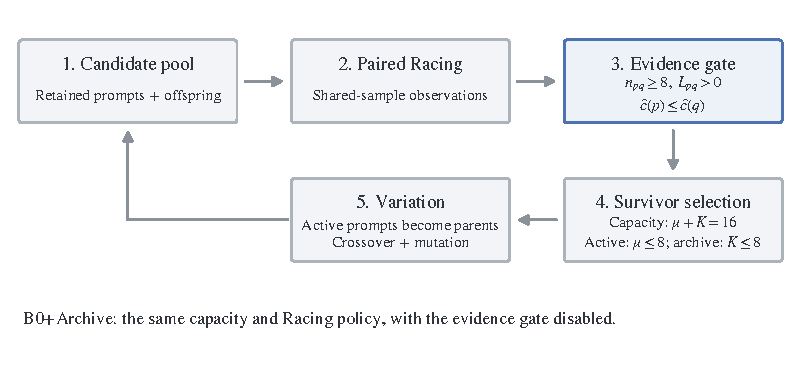
\includegraphics[width=\linewidth]{method_overview.pdf}
\caption{Survival within the evolutionary loop. The online control uses the same
Paired Racing policy and total retention capacity, with the evidence gate disabled.
Actual purchased evaluations may diverge as the two searches retain different prompts.
The evaluator also keeps historical IDs, as detailed in Section~\ref{sec:algorithm}.}
\label{fig:method}
\end{figure}

\paragraph{Survivor procedure.}
Table~\ref{tab:algorithm} gives the implemented selection procedure. The gate is
sequential: an already removed candidate is skipped as a potential dominator.
This ordering prevents a deleted prompt from supplying a later elimination
certificate, but it also means the procedure is not an order-invariant batch
solution to all possible pairwise inequalities. Stable prompt IDs make the
chosen order reproducible. They do not provide an optimality guarantee.

\begin{table}[tbp]\centering\small
\caption{PACE survivor procedure. This is pseudocode for one invocation, not the
complete evaluation scheduler. $\operatorname{NSGA}(R,k)$ denotes rank/crowding
selection of at most $k$ prompt IDs from $R$.}
\label{tab:algorithm}
\begin{tabularx}{\linewidth}{@{}r>{\raggedright\arraybackslash}X@{}}\toprule
Step & Operation\\\midrule
1 & Input candidate IDs $C$, observed state, active capacity $\mu$, archive allowance
$K$, threshold $\varepsilon$, and seeded bootstrap generator. Set $E=\varnothing$.\\
2 & Visit $q$ in sorted $C$. Visit $p$ in sorted $C$, skipping $p=q$ and IDs in $E$.\\
3 & Skip the pair if $\widehat c(p)>\widehat c(q)$, if no common samples exist,
or if fewer than eight common samples are available.\\
4 & If $L_{pq}>\varepsilon$, append $(q,p,L_{pq},U_{pq},n)$ to the confidence log,
set $E\leftarrow E\cup\{q\}$, and stop scanning dominators for $q$.\\
5 & Set $R=C\setminus E$. If $|R|>\mu+K$, keep $\operatorname{NSGA}(R,\mu+K)$
and log all other IDs as forced evictions.\\
6 & If $|R|>\mu$, set $A=\operatorname{NSGA}(R,\mu)$; otherwise set $A=R$.
Return retained set $R$, active set $A$, and the two removal logs.\\\bottomrule
\end{tabularx}
\end{table}

The control B0+Archive executes the same capacity and active-set steps with
$E=\varnothing$. In contrast, archive-free B0 directly truncates to $\mu$.
Consequently, disabling the gate while retaining $K=8$ is the relevant primary
control, whereas comparing PACE against archive-free B0 changes two components.
Setting $K=0$ removes headroom but does not logically disable evidence-based
elimination; the gate can still change which candidates reach NSGA-II truncation.
Any similarity under that ablation is an observation, not an identity of the rules.

An invocation can return fewer than $\mu$ active prompts if confidence elimination
leaves too few candidates. The implementation does not repopulate the set with
eliminated IDs to fill empty slots. This detail matters when interpreting
population size as an upper bound rather than an invariant count at every phase.
Likewise, a candidate retained in the archive is not automatically selected as a
parent: only the active set enters the variation operator.

\subsection{Variation operators and representation constraints}
Each instruction contains a literal \texttt{\{text\}} placeholder, which is
replaced with the article at evaluation time. The online initial population is
\texttt{p00}, \texttt{p01}, \texttt{p02}, \texttt{p03}, \texttt{p04},
\texttt{p05}, \texttt{p07}, and \texttt{p15}. This eight-prompt population is a
subset of the 16-prompt pool used in offline replay; the two pools should not be
conflated when assessing what candidates were available.

For each child, two parent IDs are sampled with replacement from the active
population. With probability one half, crossover combines an instruction head
from one parent with a response-format tail from the other, splitting at the
placeholder. Otherwise, the first parent's text is copied. Every child then
receives one of five uniformly chosen mutation types: replace or add a role
prefix; alter the response-format suffix; add a label-definition sentence;
make a small wording substitution; or shorten the instruction using line-based
chunks. Placeholder repair appends an article field when needed.

These operations generate readable strings without extra LLM calls. They are
intended to preserve the task and label vocabulary, but they do not prove semantic
equivalence or grammatical quality. Repeated prefixes, incomplete definitions,
and conflicting response instructions can occur. Distinct child IDs can also
contain identical strings because there is no text-level deduplication. This
restricted operator family keeps the search easy to inspect, while
limiting conclusions about stronger LLM-generated mutations or general prompt
optimization systems.

\subsection{Evaluation scope and computational complexity}
A survivor invocation considers at most $m(m-1)$ directed candidate comparisons.
If $n$ is the typical common-sample count and $B=200$, a straightforward upper
bound for bootstrap arithmetic is $O(m^2Bn)$, in addition to maintaining
observations and sorting fronts. Cost checks, previously eliminated IDs and
minimum-sample checks reduce the comparisons that proceed to a usable decision.
The implementation is intended for small pools; no wall-clock overhead benchmark
is available, so a call-neutral gate should not be described as computationally
free.

There is also an implementation distinction between the survivor pool and the
evaluation registry. The search state accumulates IDs of generated prompts;
adding children does not remove historical IDs from that registry. The Racing
policy constructs contenders from this state, while survivor selection receives
the current retained prompts and new offspring. Thus, a removed prompt can
remain visible to subsequent evaluation allocation without being eligible to
breed or become the final winner. The present results describe that exact
implementation. Pruning evaluation eligibility to the current survivor pool
would change budget allocation and requires a new experiment, not a retrospective
reinterpretation of these logs.


\section{Experimental Design}
\subsection{Configuration, data and output interpretation}
\label{sec:data-protocol}
Experiments use a single NVIDIA A100 80GB with Qwen2.5-7B-Instruct (BF16, greedy decoding, eight maximum new tokens) on four-class AG News. A fixed manifest defines 160 search instances and 200 held-out test instances. The initial prompt pool and split are frozen; the search cap is 1,280 calls, four generations, $\mu=8$, $K=8$, minimum shared observations 8, and 200 bootstrap replicates. The online primary comparison contains 15 paired seeds: 42, 123, 456, 6707, 2026, 31415, 27182, 16180, 90210, 13579, 86753, 24680, 97531, 11235, 42424. The first three were exploratory; the remaining 12 form the subsequently planned extension. The extension was planned after the exploratory results were available. Its interval describes the combined 15-seed sample; it does not account for that decision to extend the study.

\paragraph{Dataset construction and output interpretation.}
The frozen manifest contains 40 search examples per class and 50 held-out examples
per class. Search articles come from the AG News training split and held-out
articles from its test split. The four class names are World, Sports, Business,
and Sci/Tech. Disjointness is checked both by stored sample IDs and by
source-split/index pairs. Stratification controls class counts in these small
samples, but does not remove all variation in article difficulty or topic mix.
The reported accuracy is ordinary micro-accuracy on a class-balanced fixed set;
per-class errors are not reconstructed from the winner summaries.

Each rendered prompt is supplied as a user message through the target model's
chat template, with a generation prompt added. Greedy decoding and an eight-token
output cap are used throughout. The parser examines the first output line,
limited to 80 characters, attempts to extract a label field if present, and
matches a fixed set of label patterns. Its pattern order is Sci/Tech, Sports,
Business, then World; a numeric label from one to four is a fallback. Outputs
that cannot be parsed are counted as incorrect. Measured fitness
reflects the combination of instruction, model response, decoding cap and parser,
rather than abstract classification ability independently of response format.

This interaction is relevant for the format-oriented prompts. A request for JSON
or explanatory text can consume the short output allowance, while the parser
accepts some variants beyond the canonical label strings. Changing the parser or
the decoding limit after seeing results would change the evaluation task. The
current study holds them fixed and does not infer that a longer explanation
would improve or worsen accuracy on this data.


\subsection{Baselines and experimental questions}
\textbf{Offline (Gate 1):} Point-estimate NSGA-II truncation versus PACE under the same frozen 16-prompt matrix and shared evaluation purchases. The full matrix is accessible only to an offline auditor for reference-Pareto labels. Let $P^\star$ be the non-dominated prompt IDs under accuracy and token cost
computed from the complete frozen \emph{search} matrix, and let $R$ be the retained
set. The false-elimination rate is
$|P^\star\setminus R|/|P^\star|$ and reference-Pareto recall is
$|P^\star\cap R|/|P^\star|$. These are complementary measures on this finite
reference, not labels of population-level optimality.

\textbf{Online (Gate 2):} The primary comparison is \emph{PACE versus B0+Archive} with matched total capacity $\mu+K=16$, seeds, search cap, evaluation policy, and test procedure. The older B0 point-estimate variant has no auxiliary archive and is illustrative, not the primary fair contrast. Ablations disable the gate (A1), remove archive headroom ($K=0$), or remove the Gate-1 warm cache. We do not treat these ablations as confirmatory multiple-hypothesis tests.

\subsection{Racing policy and generation schedule}
The evaluation policy first constructs up to six contenders using the estimated
non-dominated front and nearby candidates. It considers up to eight neighboring
pairs after ordering by estimated cost. Paired uncertainty is summarized by a
bootstrap utility-ranking reversal rate. Among eligible pairs, the policy scores
reversal rate per expected additional observation, with an observation-count
fallback when all scores are zero. The stop threshold is 0.05. Selected pairs
receive up to eight randomly chosen shared examples that neither member has yet
observed. When no eligible pair query is returned, the policy attempts to buy a
common sample column for the registered prompt IDs.

Racing and survival use different evidence questions. Racing asks where another
observation might alter a utility ranking. The PACE gate asks whether a prompt
has enough paired accuracy evidence to justify removal at no greater estimated
cost. They share observations and bootstrap machinery, but neither statistic is
a substitute for the other. Holding Racing fixed makes survival the experimental
entry point; it does not imply that all future contender sets remain identical.

The online loop has four generations and three offspring rounds. It initializes
the eight prompts on eight shared examples, allocates part of the remaining
budget to Racing, and selects survivors. Before the next generation it generates
eight children, warms them on up to four shared examples, evaluates again, and
selects from retained prompts plus children. At the end, any usable residual
budget is offered to Racing before the final utility-based winner is selected.
This produces seven ordinary survivor checkpoints per run: four after the
generation-level Racing phase and three after offspring evaluation. Residual
allocation, if logged, is not an additional offspring round.

\subsection{Three resource accounts}
\label{sec:accounting}
The reported search counter increments when a previously unobserved
prompt--sample pair is entered into the run's search state. Requesting the same
observed pair again costs zero in this counter. A separate predictor-level inference
cache may already contain that result, including entries imported from the
Gate-1 matrix for initial prompts. Revealing such a result to a fresh search
state still advances the search counter even though no new GPU generation is
needed. The 1,280 limit is a cap on newly acquired \emph{search
observations}, not a measured number of physical cache misses across the machine.

Deployment cost is the mean recorded input-plus-output token count of the selected
winner on the 200 held-out examples. Input counts use the attention mask to exclude
left-padding tokens; generated padding is excluded when possible, with at least
one output token recorded. These values describe the inference format used here,
including chat-template overhead. They are not a monetary price or a hardware
latency estimate. Held-out winner evaluation is separate from the search budget;
bootstrap calculations, cache lookups and mutation operations are also outside
that observation counter.

\subsection{Inference across seeds}
Let $\delta_s$ be PACE accuracy minus control accuracy for paired seed $s$.
The primary estimator and reported Student-$t$ interval are
\begin{equation}
 \bar\delta=\frac{1}{15}\sum_{s=1}^{15}\delta_s,\qquad
 \bar\delta\pm t_{0.975,14}\frac{s_\delta}{\sqrt{15}}.
 \label{eq:seed-interval}
\end{equation}
The stored report uses the rounded critical value 2.145. The paired sign-flip
analysis samples 100,000 independent sign vectors with a fixed random seed and
compares absolute null means with $|\bar\delta|$. This is a Monte Carlo
randomization-style check on paired differences, relying on a suitable sign
symmetry/exchangeability interpretation under the null. It is not a randomized
assignment of prompts to independent test populations.

The nominal interval does not incorporate uncertainty from the decision to extend
the study after the original three seeds. Nor does pairing turn the shared 200
test articles into 3,000 independent held-out examples. Every winner is judged
on that same article set. We retain the original seeds, identify them explicitly,
and distinguish descriptive sensitivity checks from the primary estimate.


\section{Results}
\subsection{Offline elimination reliability}
\begin{table}[tbp]\centering\small\caption{Gate 1 at evaluation budget 640 (20 replay seeds, same frozen model-response matrix). Lower false-elimination rate is better.}\begin{tabular}{lrrr}\toprule
Method & False elimination & Reference-Pareto recall & Retained-set regret\\\midrule
Point-estimate NSGA-II ($\mu=8$) & 0.183 & 0.817 & 0.0007\\
PACE ($\mu=8,K=8$) & \textbf{0.025} & \textbf{0.975} & \textbf{0.0000}\\\bottomrule\end{tabular}\end{table}
\begin{figure}[tbp]\centering
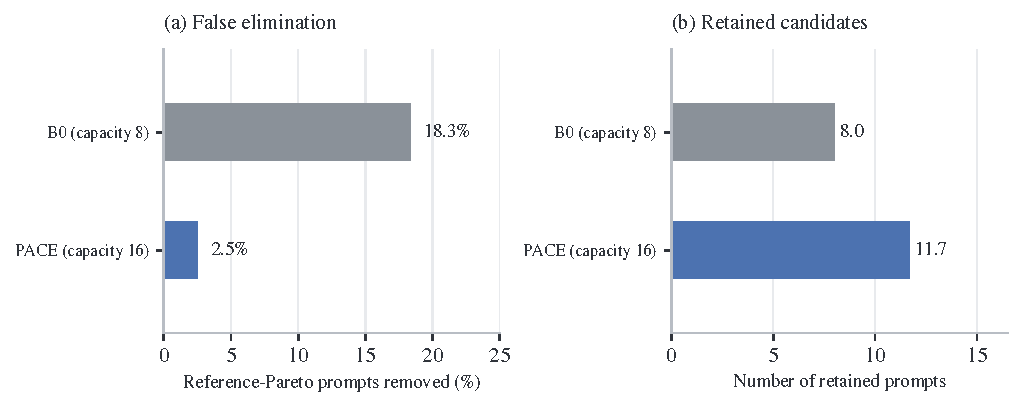
\includegraphics[width=\linewidth]{offline_replay.pdf}
\caption{Offline replay at budget 640. Bars show means across 20 replay seeds:
(a) false elimination of reference-Pareto prompts and (b) actual retained-set size.
Capacity limits are 8 for B0 and 16 for PACE. All seeds use the same frozen
prediction matrix. Descriptive variability at both budgets is shown in
Figure~\ref{fig:budgets}.}
\label{fig:gate1}
\end{figure}
PACE retains more reference-Pareto prompts in the offline replay (Fig.~\ref{fig:gate1}). It also has twice the retention capacity, so this comparison measures the combined gate-and-archive effect. The 20 replay seeds vary the observation trajectory on one frozen matrix; they do not represent 20 independent datasets or model evaluations.

\subsection{Capacity-matched online comparison}
\begin{table}[tbp]\centering\caption{Gate 2 primary result: 15 paired online seeds, 200 held-out test examples per winner.}\begin{tabular}{lrrrr}\toprule
Method & Test accuracy & Tokens/example & Search calls & Budget use\\\midrule
B0 + Archive & 78.4\% & \textbf{112.6} & 1275 & 99.6\%\\
PACE & \textbf{80.1\%} & 115.5 & 1276 & 99.7\%\\\bottomrule\end{tabular}\end{table}
\begin{figure}[tbp]\centering
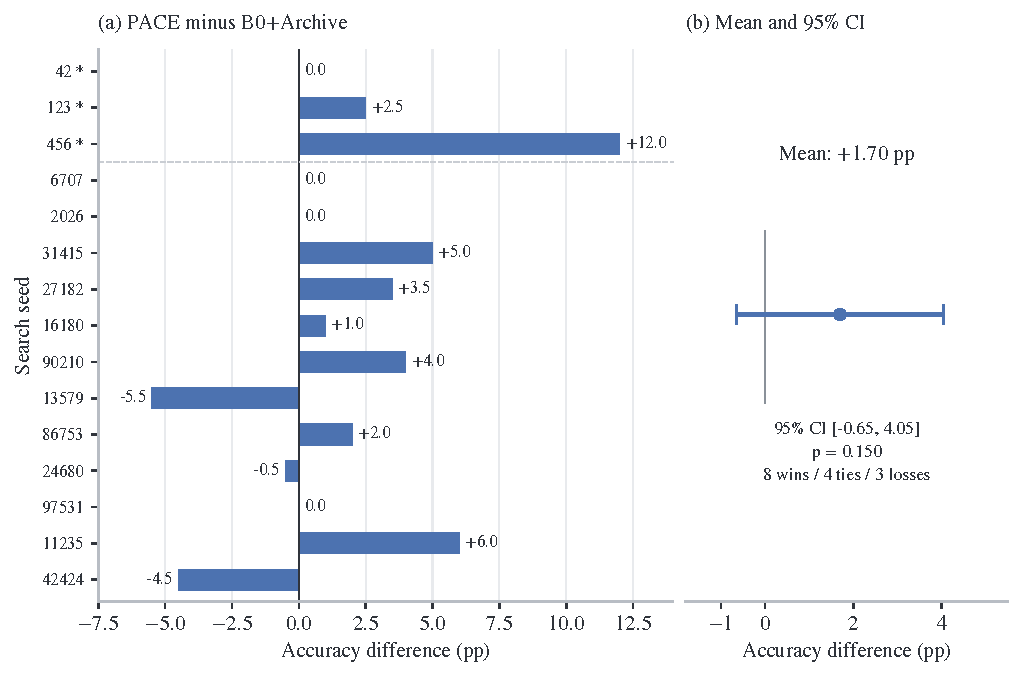
\includegraphics[width=\linewidth]{online_paired.pdf}
\caption{Capacity-matched online accuracy differences (PACE minus B0+Archive).
(a) Bars show all 15 paired differences in protocol order, including ties.
Asterisks and the horizontal divider identify the first three exploratory seeds. (b) Mean paired difference and Student-$t$ 95\% interval across
search seeds. The interval crosses zero; the experiment does not establish
an online accuracy advantage.}
\label{fig:paired}
\end{figure}
The paired average is $\Delta\mathrm{accuracy}=+0.0170$ (+1.70 percentage points). A Student-$t$ interval for the 15 paired seed differences is $[-0.0065,0.0405]$, i.e., $[-0.65,4.05]$ percentage points; the two-sided paired sign-flip permutation test gives $p\approx0.150$. Win/tie/loss counts are 8/4/3. The estimated difference is positive, but the interval includes zero. The mean deployment-token increase is approximately 2.6\%. The outcomes also vary markedly by seed, including both substantial PACE gains and losses (Fig.~\ref{fig:paired}). Figure~\ref{fig:paired}(b) shows uncertainty in the mean effect.
Figure~\ref{fig:cost} displays the accompanying accuracy--cost trade-off.

\subsection{Focused ablations}
\begin{table}[tbp]\centering\small\caption{Exploratory three-seed ablation means; these are not replacements for the 15-seed primary contrast.}\begin{tabularx}{\linewidth}{@{}lrrX@{}}\toprule
Comparison & Baseline acc. & Treatment acc. & Interpretation\\\midrule
Original PACE vs point B0 & 0.783 & 0.810 & Confounded by archive capacity\\
PACE with $K=0$ vs B0 & 0.783 & 0.782 & No gain without archive headroom\\
Gate disabled (A1) vs B0 & 0.783 & 0.787 & Near point-estimate behavior\\
Cold-start PACE vs cold B0 & 0.787 & 0.802 & Small positive exploratory difference\\\bottomrule\end{tabularx}\end{table}
The primary comparison holds archive capacity fixed, so its point estimate
reflects the complete trajectory change induced by enabling the gate. Its
uncertainty prevents concluding that gating improves online accuracy.
Forced capacity evictions remain frequent. Logs indicate that a substantial fraction of archive-only prompts later enter the active breeding set, while many archive slots are occupied by candidates that do not subsequently breed. In the archive-only transition audit, 52\% later appeared in the active set before an offspring step (a proxy for breeding opportunity), while never-breeding candidates accounted for approximately 46.5\% of archive-slot steps. These descriptive counts do not prove beneficial descendant production. Missing parent IDs preclude precise lineage-based causal claims.

\begin{figure}[tbp]\centering
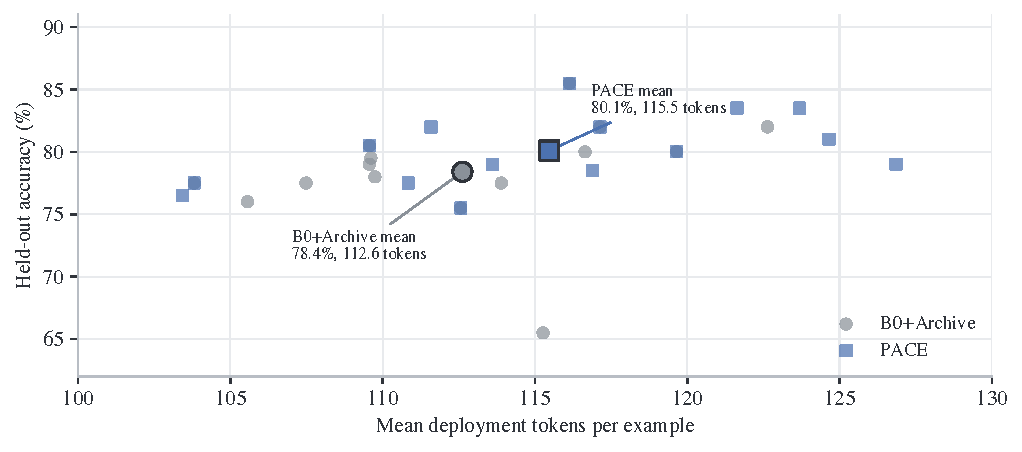
\includegraphics[width=\linewidth]{accuracy_cost.pdf}
\caption{Held-out accuracy and deployment-token cost of selected winners.
Gray circles show B0+Archive and blue squares show PACE. Small symbols are
individual runs; outlined symbols mark method means. Higher accuracy and lower
cost are preferred.}
\label{fig:cost}
\end{figure}

\section{Detailed results and mechanism analysis}
\label{sec:extended}
\subsection{Offline behavior at both recorded budgets}
The replay configuration records budgets 320 and 640. Figure~\ref{fig:budgets}
shows both, retaining budget 640 as the primary offline result. Each point
aggregates 20 policy trajectories on the same frozen 16-by-160 correctness and
token matrix. The comparison reuses one observation state for the two survivor
rules at a given budget and seed; unlike the online experiment, there is no
subsequent divergence in candidate generation.

\begin{figure}[tbp]\centering
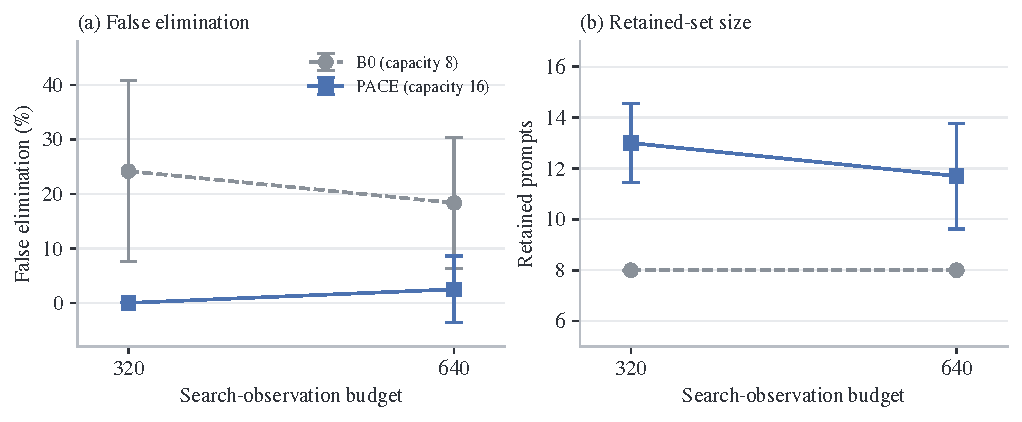
\includegraphics[width=\linewidth]{replay_budgets.pdf}
\caption{Offline replay across the two recorded budgets. Points and error bars
are means and $\pm1$ sample standard deviation across 20 replay seeds. Left:
false-elimination rate. Right: retained-set size. The unequal capacity limits
remain part of the comparison at both budgets; lines only join recorded settings.}
\label{fig:budgets}
\end{figure}

Increasing the observation budget changes the evidence available for the gate
and can alter estimated fronts. It does not remove the retention-capacity
confound: PACE can keep up to all 16 original prompts, whereas archive-free B0
must discard eight. The appropriate interpretation is therefore that the combined
configuration changes finite-pool retention, not that the graph estimates an
isolated causal effect of a calibrated confidence procedure.

The retained-set regret in the offline table is an audit utility gap. An auditor
uses full search-matrix estimates to choose the best retained prompt and compares
it with the best prompt in the complete frozen pool under the same fixed utility.
This differs from the online procedure, where the winner is chosen using partial
search observations and only that winner receives a held-out evaluation. A zero
offline retained-set regret means that at least one utility-optimal reference
candidate remains available; it does not imply that every Pareto candidate was
retained or that a noisy final selector would choose the oracle-preferred one.

\subsection{Search trajectories and capacity pressure}
Figure~\ref{fig:dynamics} summarizes cumulative observation acquisition and
retained-set size at the seven survivor checkpoints. Both methods approach the
same observation cap, yet their candidate counts need not coincide. PACE can
remove a prompt before the set exceeds capacity, while the control only removes
prompts through rank/crowding truncation. Similar total budgets therefore do not
imply identical allocation among candidates or equal information per survivor.

\begin{figure}[tbp]\centering
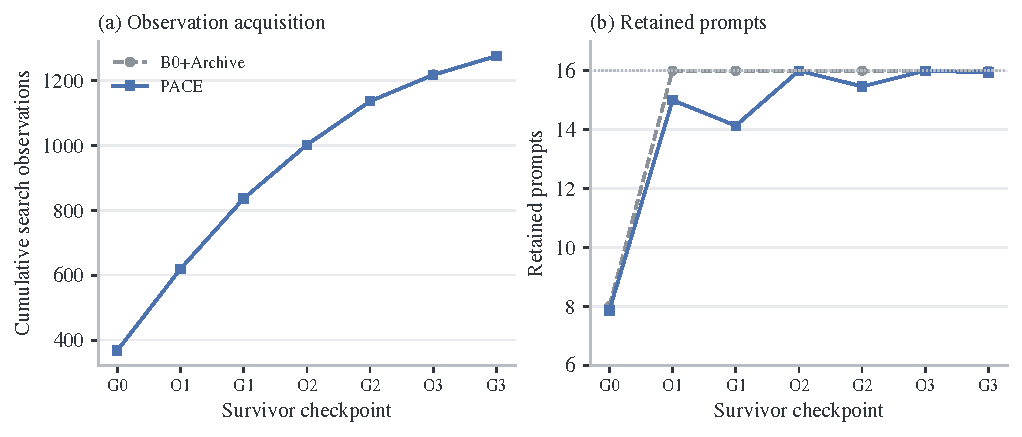
\includegraphics[width=\linewidth]{search_dynamics.pdf}
\caption{Mean online trajectories across 15 paired seeds. Checkpoints alternate
between generation Racing ($G$) and offspring evaluation ($O$); lines show the method means. Left: cumulative acquired search observations.
Right: retained candidate count. Counts are measured after survival; the dashed
line is the matched total capacity of 16. No intermediate test accuracy is implied.}
\label{fig:dynamics}
\end{figure}

The logs allow a description of removal decisions without assigning each removal
a counterfactual value. PACE has 3.80 confidence eliminations and 12.27 forced
evictions per run on average, compared with zero and 16.00 for B0+Archive.
The audit's mean per-run forced-removal share is 0.765 for PACE. This is a mean
of ratios and should not be confused with the ratio of the two mean counts.
The confidence gate relocates some decisions, but forced capacity decisions
still account for most recorded removals.

\begin{table}[tbp]\centering\small
\caption{Descriptive archive audit of the 15 primary paired runs. Search accuracy
is computed on observed search data; it is not an additional held-out score.
Transition rates are proxies derived from active/retained IDs.}
\label{tab:archive}
\begin{tabularx}{\linewidth}{@{}>{\raggedright\arraybackslash}Xrr@{}}\toprule
Signal & B0+Archive & PACE\\\midrule
Confidence eliminations per run & 0.00 & 3.80\\
Forced evictions per run & 16.00 & 12.27\\
Mean within-run forced-removal share & 1.000 & 0.765\\
Never-breeding share of archive-slot steps & 0.436 & 0.465\\
Archive-only IDs later active before offspring & 0.555 & 0.520\\
Mean final archive search accuracy & 0.755 & 0.787\\
Mean final active search accuracy & 0.762 & 0.769\\
Runs whose winner was ever archive-only & --- & 0.200\\\bottomrule
\end{tabularx}
\end{table}

Table~\ref{tab:archive} shows why archive occupancy is not equivalent to productive
protection. Roughly half of archive-only IDs later become active before an
offspring step, but a substantial portion of archive-slot occupancy belongs to
IDs that never do so. The two rates have different denominators: one counts
candidate transitions and the other counts occupied slots over time. They need
not sum to one. Final archive search accuracy is not lower than final active
accuracy for PACE, which also argues against interpreting every unused archive
slot as obviously poor. Selection, sample counts and observation histories all
affect those descriptive averages.

\subsection{Sensitivity to the exploratory cohort and individual seeds}
\label{sec:sensitivity}
The first three paired seeds contribute a mean difference of 4.83 percentage
points, whereas the subsequent 12 contribute 0.92 points. Their weighted mean is
1.70 points. Figure~\ref{fig:sensitivity} makes this decomposition visible and
shows leave-one-seed-out means. These are post-hoc descriptions of the existing
runs, not new confirmatory experiments or alternative primary analyses.

\begin{figure}[tbp]\centering
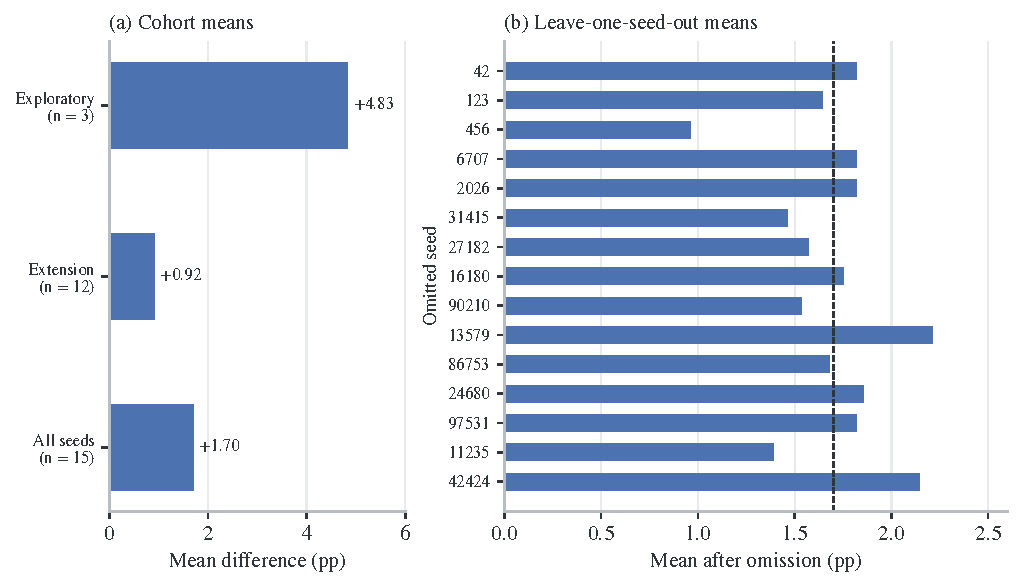
\includegraphics[width=\linewidth]{seed_sensitivity.pdf}
\caption{Descriptive sensitivity analysis. Left: cohort means and sample sizes,
with no inferential error bars. Right: means after omitting each paired seed in
turn, in protocol order. The dashed reference is the full 15-seed mean. Omission
is diagnostic only; no seed is excluded from the primary analysis.}
\label{fig:sensitivity}
\end{figure}

The largest individual gain is 12.0 percentage points at seed 456, and the largest
loss is 5.5 points at seed 13579. Omitting one seed at a time yields means from
0.96 to 2.21 points. This is the range of omission means, not a confidence interval. A positive mean throughout these omissions does
not overturn the primary interval crossing zero. The extension-only mean is
likewise not independent replication across tasks: it uses the same fixed model,
manifest, operators and held-out examples.

\subsection{Contrasting winner examples}
For seed 456, the control winner achieves 65.5\% and the PACE winner 77.5\%.
The control text contains an abbreviated definition header, while the PACE text
combines a librarian role with an explicit single-label instruction. For seed
13579, the control achieves 82.0\% and PACE 76.5\%, with the control using a
longer canonical-label format instruction. Exact strings appear in
Appendix~\ref{app:prompts}. These cases show that the same operator family can
produce both gains and losses; they do not establish a general rule that roles,
length, or a particular wording cause better classification.

Seed 42 is a useful contrast: both searches select exactly the same instruction
string and reach 85.5\% accuracy, even though generated IDs carry different method
prefixes. An unchanged winner can coexist with different survival logs. Changes in the survivor logs can therefore occur without changing the
selected instruction. The winner-only evaluation protocol supports these endpoint
comparisons, but does not provide class-level explanations, per-example paired
error tests, or a held-out trajectory for every generated candidate.


\section{Discussion and limitations}
\label{sec:limitations}
\paragraph{Retention is an intermediate outcome.}
The detailed audit separates evidence-based removal, capacity pressure and
archive reuse. Better retention on a finite reference pool need not produce a
better final instruction: the retained prompts must still receive useful
evaluations or contribute to productive variation. The matched online comparison
addresses the complete trajectory effect, while incomplete parent logging leaves
the value of individual archive events unresolved.

\paragraph{What the online interval measures.}
The inferential unit is a paired \emph{search seed}. The 95\% interval allows both
a small disadvantage and a meaningful advantage on the fixed task and test set.
The two-sided sign-flip test is also inconclusive. All runs share the same 200
test examples, so adding seeds primarily measures search stochasticity rather
than uncertainty over new test populations. The first three seeds had an
exploratory mean gain of 4.83 percentage points. The 15-seed extension retains
those observations and yields the smaller 1.70-point estimate; it is not an
independent, blinded confirmation. The ablations use only three seeds and
support descriptive comparisons rather than confirmatory hypothesis tests.

\paragraph{The confidence gate is a heuristic.}
With as few as eight common observations, percentile bootstrap intervals can
be unstable. When all observed paired differences coincide, the implemented
interval collapses to a point. Repeated adaptive pair comparisons with 200
resamples have no simultaneous or anytime-valid coverage guarantee. Token
costs enter as point estimates, without uncertainty adjustment. Here, ``confidence-preserving'' names the removal rule. Sampling errors and
forced evictions can still remove competitive prompts.

\paragraph{Scope and computational accounting.}
The study uses one dataset, one target model, a small population, and rule-based
variation. It does not establish generalization to other tasks or LLMs. The
1,280-observation cap measures new acquisitions into the run state, not physical GPU cache misses or wall-clock time,
bootstrap computation, or the separate winner-only test evaluation. The reported
deployment tokens also measure a different resource from acquired search observations.
Earlier DICE allocation experiments are archived separately and excluded from
the PACE estimate. The analysis uses the recorded runs throughout.

\section{Conclusion}
PACE combines paired-evidence elimination with a bounded archive in budgeted
multi-objective prompt search. On the frozen offline pool, the combined
intervention reduced false elimination, with retention capacity contributing
to the contrast. At matched online capacity, the mean accuracy improvement was
1.70 percentage points and deployment-token cost increased by approximately
2.6\%; the confidence interval includes zero. These results justify further
study of survivor decisions, while leaving the downstream accuracy advantage
unresolved. The next tests should retain matched capacities, use independent
tasks and test samples, and add calibrated sequential evidence and complete
parent-lineage logs.

\section*{Code and data}
Code, configurations, split manifests and recorded results are available at
\url{https://github.com/moonriver0922/DSAI6707-PACE}. The repository README gives
installation, figure-generation and replay instructions. The survivor rule is
implemented in \path{src/pace/}; the online configuration is
\path{configs/pace_gate2_cap_align_15seed.yaml}. The 30 primary run records and
paired summaries are under \path{outputs/pace/gate2_cap_align_15seed/}.
Figures are generated directly from these files. The held-out data are listed
in \path{data/split_manifest.json}; full inference requires the specified model
and a compatible CUDA environment. The analysis here reuses stored results.
The repository also preserves earlier DICE experiments under separate paths.

\begin{thebibliography}{99}\small
\bibitem{evoprompt} Guo et al. (2024). Connecting Large Language Models with Evolutionary Algorithms Yields Powerful Prompt Optimizers. \emph{ICLR}. \url{https://proceedings.iclr.cc/paper_files/paper/2024/hash/9156b0f6dfa9bbd18c79cc459ef5d61c-Abstract-Conference.html}.
\bibitem{promptbreeder} Fernando, C., Banarse, D. S., Michalewski, H., Osindero, S., and Rockt"{a}schel, T. (2024). Promptbreeder: Self-Referential Self-Improvement via Prompt Evolution. \emph{ICML}. \url{https://proceedings.mlr.press/v235/fernando24a.html}.
\bibitem{capo} Zehle, T., Schlager, M., Hei\ss, T., and Feurer, M. (2025). CAPO: Cost-Aware Prompt Optimization. \emph{AutoML}. \url{https://proceedings.mlr.press/v293/zehle25a.html}.
\bibitem{mocapo} B\"ussing, J., Schlager, M., Hei\ss, T., Zehle, T., and Feurer, M. (2026). MO-CAPO: Multi-Objective Cost-Aware Prompt Optimization. \emph{arXiv:2605.18869}. \url{https://arxiv.org/abs/2605.18869}.
\bibitem{gepa} Agrawal, L. A., et al. (2026). GEPA: Reflective Prompt Evolution Can Outperform Reinforcement Learning. \emph{ICLR}. \url{https://proceedings.iclr.cc/paper_files/paper/2026/hash/0e9e708b6f48e14fd0ac29e167413f76-Abstract-Conference.html}.
\bibitem{opro} Yang et al. (2024). Large Language Models as Optimizers. \emph{ICLR}. \url{https://arxiv.org/abs/2309.03409}.
\bibitem{opro_revisit} Zhang, Yuan, and Avestimehr (2024). Revisiting OPRO: The Limitations of Small-Scale LLMs as Optimizers. \emph{Findings of ACL}. \url{https://aclanthology.org/2024.findings-acl.100/}.
\bibitem{instructzero} Chen, L., Chen, J., Goldstein, T., Huang, H., and Zhou, T. (2024). InstructZero: Efficient Instruction Optimization for Black-Box Large Language Models. \emph{ICML, PMLR 235:6503--6518}. \url{https://proceedings.mlr.press/v235/chen24e.html}.
\bibitem{promptwizard} Agarwal, E., Magazine, R., Singh, J., Dani, V., Ganu, T., and Nambi, A. (2025). PromptWizard: Optimizing Prompts via Task-Aware, Feedback-Driven Self-Evolution. \emph{Findings of ACL}. \url{https://aclanthology.org/2025.findings-acl.1025/}.
\bibitem{riot} Zhou et al. (2025). RiOT: Efficient Prompt Refinement with Residual Optimization Tree. \emph{ACL}. \url{https://aclanthology.org/2025.acl-long.1086/}.
\bibitem{survey_li} Li, W., Wang, X., Li, W., and Jin, B. (2025). A Survey of Automatic Prompt Engineering: An Optimization Perspective. \emph{arXiv:2502.11560}. \url{https://arxiv.org/abs/2502.11560}.
\bibitem{survey_cui} Cui, W., Li, Z., Sun, H., Lopez, D., Das, K., Malin, B. A., Kumar, S., and Zhang, J. (2025). A Survey of Automatic Prompt Optimization with Instruction-focused Heuristic-based Search Algorithm. \emph{arXiv:2502.18746}. \url{https://arxiv.org/abs/2502.18746}.
\bibitem{survey_ramnath} Ramnath, K., et al. (2025). A Systematic Survey of Automatic Prompt Optimization Techniques. \emph{EMNLP}. \url{https://aclanthology.org/2025.emnlp-main.1681/}.
\bibitem{budgetapo} Liu, H., Wang, Z., Yan, H., and Tang, X. (2026). How Should a Prompt Optimizer Spend a Tight Budget? BudgetAPO with Noise-Adaptive Evaluation. \emph{arXiv:2610.05671}. \url{https://arxiv.org/abs/2610.05671}.
\bibitem{ipomp} Dong, X., Wang, S., Lin, D., and Hassan, A. (2025). Model Performance-Guided Evaluation Data Selection for Effective Prompt Optimization. \emph{Findings of ACL}, pp. 2844--2859. \url{https://aclanthology.org/2025.findings-acl.147/}.
\bibitem{probsel} Yang, S., Kim, J., Jang, J., Ye, S., Lee, H., and Seo, M. (2024). Improving Probability-based Prompt Selection Through Unified Evaluation and Analysis. \emph{TACL}. \url{https://aclanthology.org/2024.tacl-1.37/}.
\bibitem{iapo} Mahmud, S., Nakamura, M., Wray, K. H., and Zilberstein, S. (2026). Inference-Aware Prompt Optimization for Aligning Black-Box Large Language Models. \emph{AAAI 40(38):32455--32464}. \url{https://ojs.aaai.org/index.php/AAAI/article/view/40521}.
\bibitem{autopdl} Spiess, C., Vaziri, M., Mandel, L., and Hirzel, M. (2025). AutoPDL: Automatic Prompt Optimization for LLM Agents. \emph{arXiv:2504.04365}. \url{https://arxiv.org/abs/2504.04365}.
\bibitem{toolbox} Grie{\ss}haber, D., Kimmich, M., Maucher, J., and Vu, T. (2025). A Toolbox for Improving Evolutionary Prompt Search. \emph{Proceedings of the 2nd LUHME Workshop}, pp. 58--66. \url{https://aclanthology.org/2025.luhme-1.6/}.
\bibitem{depth} Wang, S., and Lu, Z. (2026). Depth over Fidelity in Fixed-Budget Noisy Evolution Strategies. \emph{ICML, PMLR 306:128714--128741}. \url{https://proceedings.mlr.press/v306/wang26ff.html}.
\bibitem{selectionnoise} Gulayeva, N. M., Borrego-Diaz, J., and Sancho-Caparrini, F. (2025). Analysis of Selection Noise in Genetic Algorithms. \emph{Soft Computing 29:3757--3773}. \url{https://link.springer.com/article/10.1007/s00500-025-10652-6}.
\bibitem{robotnoise} Martin and Collins (2026). Improving CMA-ES Convergence Speed, Efficiency, and Reliability in Noisy Robot Optimization Problems. \emph{Evolutionary Computation}. \url{https://pubmed.ncbi.nlm.nih.gov/41604289/}.
\bibitem{evalbefore} Sadjoli et al. (2025). Optimization before Evaluation: Evaluation with Unoptimized Prompts Can Be Misleading. \emph{ACL Industry}. \url{https://aclanthology.org/2025.acl-industry.44/}.
\bibitem{nsga2} Deb et al. (2002). A Fast and Elitist Multiobjective Genetic Algorithm: NSGA-II. \emph{IEEE Transactions on Evolutionary Computation}.
\end{thebibliography}

\clearpage
\appendix
\section{Implementation and reporting details}
\label{app:details}
\begin{table}[htbp]\centering\small
\caption{Frozen online configuration. Search and held-out evaluation use disjoint
manifest IDs. Costs in the final winner utility use the fixed normalization
in Equation~\ref{eq:winner}.}
\begin{tabularx}{\linewidth}{@{}lX@{}}\toprule
Setting & Value\\\midrule
Task and target model & AG News; Qwen2.5-7B-Instruct\\
Search / held-out examples & 160 / 200\\
Decoding & BF16; greedy; maximum 8 new tokens\\
Active / archive capacity & $\mu=8$, $K=8$ for both primary methods\\
Initial / generated prompts & 8 initial; 24 offspring across 3 variation rounds\\
Search schedule & 4 generations, Paired Racing, at most 1,280 search observations\\
Shared anchor / offspring warm-up & 8 / up to 4 common examples\\
Evidence gate & $n_{\min}=8$; $\varepsilon=0$; 200 bootstrap resamples\\
Paired interval & Percentile 2.5\% and 97.5\% quantiles\\
Final preference & $\lambda=0.5$; token normalization $[0,256]$\\
Test protocol & One search-selected winner per method and seed\\\bottomrule
\end{tabularx}
\end{table}

\paragraph{Reproduction of the paper figures.}
The accompanying \path{paper/make_figures.py} reads frozen CSV/JSON outputs,
validates online accuracy values against the 30 per-run JSON files, and exports
vector PDF figures and PNG previews. It does not rerun inference or modify
experimental records. Offline plots show replay-level standard deviations,
while the online interval uses the 15 paired seed differences; these are
different uncertainty summaries.

\section{Complete paired online results}
\label{app:paired}
Table~\ref{tab:all-seeds} reports every paired endpoint in protocol order.
Accuracy is expressed as a percentage and the difference in percentage points.
Token costs are per held-out example. The first three runs are retained
exploratory observations, not repeated measurements created for the extension.
The table is generated from the same stored paired CSV used in the figures.

\begin{table}[htbp]\centering\small
\caption{All 15 paired seeds. An asterisk marks the exploratory cohort.
$\Delta a$ is PACE minus B0+Archive; $c$ denotes mean deployment tokens.}
\label{tab:all-seeds}
\begin{tabular}{@{}rrrrrrr@{}}\toprule
Seed & B0 acc. & PACE acc. & $\Delta a$ (pp) & B0 $c$ & PACE $c$ & Outcome\\\midrule
42* & 85.5 & 85.5 & +0.0 & 116.1 & 116.1 & Tie\\
123* & 77.5 & 80.0 & +2.5 & 107.5 & 119.7 & Win\\
456* & 65.5 & 77.5 & +12.0 & 115.3 & 110.8 & Win\\
6707 & 82.0 & 82.0 & +0.0 & 117.1 & 117.1 & Tie\\
2026 & 80.5 & 80.5 & +0.0 & 109.6 & 109.6 & Tie\\
31415 & 76.0 & 81.0 & +5.0 & 105.6 & 124.7 & Win\\
27182 & 80.0 & 83.5 & +3.5 & 119.7 & 123.7 & Win\\
16180 & 77.5 & 78.5 & +1.0 & 103.8 & 116.9 & Win\\
90210 & 78.0 & 82.0 & +4.0 & 109.7 & 111.6 & Win\\
13579 & 82.0 & 76.5 & -5.5 & 122.6 & 103.4 & Loss\\
86753 & 75.5 & 77.5 & +2.0 & 112.6 & 103.8 & Win\\
24680 & 79.5 & 79.0 & -0.5 & 109.6 & 126.9 & Loss\\
97531 & 79.0 & 79.0 & +0.0 & 109.6 & 113.6 & Tie\\
11235 & 77.5 & 83.5 & +6.0 & 113.9 & 121.6 & Win\\
42424 & 80.0 & 75.5 & -4.5 & 116.6 & 112.6 & Loss\\
\bottomrule\end{tabular}\end{table}

\section{Prompt examples and search-space audit}
\label{app:prompts}
The following strings are copied verbatim from the winner records. The literal
\texttt{\{text\}} placeholder is replaced by an article during evaluation.
Line wrapping is typographic only. These examples are endpoint case studies;
without complete parent logs they do not establish which earlier archive event
caused the final wording.

\paragraph{Seed 456, B0+Archive; held-out accuracy 65.5\%.}

\begin{quote}\small\ttfamily\raggedright
World=geopolitics; Sports=athletics; Business=markets; Sci/Tech=science/tech. Label definitions:\\
\{text\}\\
Label:
\end{quote}

\paragraph{Seed 456, PACE; held-out accuracy 77.5\%.}

\begin{quote}\small\ttfamily\raggedright
You are a careful news librarian. Reply with exactly one label from this set: World | Sports | Business | Sci/Tech.\\
\{text\}\\
Answer:
\end{quote}

\paragraph{Seed 13579, B0+Archive; held-out accuracy 82.0\%.}

\begin{quote}\small\ttfamily\raggedright
Valid labels: World, Sports, Business, Sci/Tech. Reply with exactly one label from this set: World | Sports | Business | Sci/Tech.\\
No extra words.\\
Article: \{text\}\\
Label:
\end{quote}

\paragraph{Seed 13579, PACE; held-out accuracy 76.5\%.}

\begin{quote}\small\ttfamily\raggedright
Classify. Category (World / Sports / Business / Sci/Tech):\\
\{text\}\\
Label:
\end{quote}

\paragraph{Initial-pool coverage.}
The offline pool has four short-direct prompts (p00, p01, p08, p12), four role
prompts (p02, p05, p10, p15), five format prompts (p03, p06, p07, p09, p14), and
three definition prompts (p04, p11, p13). The online initial subset includes two
short-direct, three role, two format and one definition prompt. These are
hand-authored categories in the frozen pool, not clusters discovered from the
reported outcomes. Evolved children may combine several categories.

\paragraph{Identity and caching.}
A prompt ID, an instruction string and a lineage are different objects.
Method-specific IDs can represent identical text, as in seed 42, while distinct
IDs are not deduplicated during mutation. Predictor-level caching uses the configured
model, prompt ID, sample ID and decoding signature. Reusing a string with a new
ID need not reuse the same cache entry. These details matter for accounting and
reproduction, but do not supply an unobserved held-out evaluation of other
candidates.


\end{document}
